\chapter{Introduction}
\label{introchap}


% what is embodied fabrication?
% what are the goals of this work? (democratization of 3d printing)

Ten years ago, 3-dimensional printing was solely the purview of large
fabrication studios and industrial manufacturing; five years ago the first
desktop ``homebrew'' 3D printers hit the market, though few people seemed to pay
much attention; today, desktop 3D printing is one of the big headlines at the
annual Consumer Electronics Showcase in Las Vegas, media outlets from
Forbes\cite{forbes} to the Economist\cite{economist} are discussing it, and most
of the teenagers we talked to during our user studies know what 3D printing is.
3D printing is part of a forceful trend often referred to as the ``maker
movement''\cite{anderson2012makers}, that puts do-it-yourself ethics and
emerging technology together in a way that has inspired people the world over to
put down the TV remote and pick up a soldering iron. A subset of this movement
has focused on ``digital fabrication'' technology, of which 3D printers, laser
cutters, CNC mills, and vinyl plotters (among other devices) belong. Digital
fabrication machines take computer-generated files as input and fabricate
physical objects from those files. With the help of the maker movement and
visionary works on the upcoming age of ``personal
fabrication''\cite{Gershenfeld:2007:FCR:1211574}, 3D printing machines that once
cost tens of thousands of dollars are now available as DIY kits for less than
one thousand. Do not misunderstand us - this is a wonderful thing; cost is one,
if not the main barrier to the spread of most technologies.
However, the maker movement is not without its blind spots. Most innovators
behind these desktop 3D printers are of a very privileged socioeconomic
background; many of them retired engineers or otherwise possessing technical
training far beyond the average person. For the most part, they have not (nor is
it necessarily their responsibility to have) truly thought about how to make
their low-cost 3D printers accessible to the average Joe and Sally - much less
Joe Jr. - and to be fair, they are not the only actors contributing to the
barrier of entry for 3D novices who wish to design for 3D printers.

For those readers who may be unfamiliar with 3D printing, it is indeed what it
sounds like - an umbrella term for one of several processes capable of creating
3-dimensional objects (usually fine layers of extruded plastic filament) from
digital files, much like a laser printer prints 2D images on paper. 3D printers
primarily take in a file format called stereolithography - or .STL for short.
Normally, to create an .STL file one needs a rather complicated,
professional-level piece of 3D-modeling software, such as Rhino\cite{Rhino} or
Solidworks\cite{Solidworks}; programs which are rich with features that only
seasoned users will find a need for, with sub-menus upon sub-menus and decidedly
particular behaviors that any novice - especially a young one - would find quite
intimidating. As anyone who has used these software programs knows, one must be
very precise and conscious of every operation for a model to turn out properly -
and this order of operations is learned slowly (often agonizingly) over time. It
is a user interface nightmare; hardly the soft of intuitive environment one
might want to learn with. It should be noted that some efforts have been made to
create entry-level 3D modeling software - most notably Google
SketchUp\cite{SketchUp} - although last we checked SketchUp did not export
directly into .STL format (there are some rather troublesome looking workarounds
however), leaving the average newcomer facing an incredibly steep learning curve
in order to produce any original, 3D-printable objects. We emphasize
``original'' because there are several fairly simple ways to download and print
out a pre-created .STL file from the Internet (most notably from the on-line
repository Thingiverse\cite{thingiverse}).

\begin{figure}[!ht]
\begin{center}$
\begin{array}{cc}
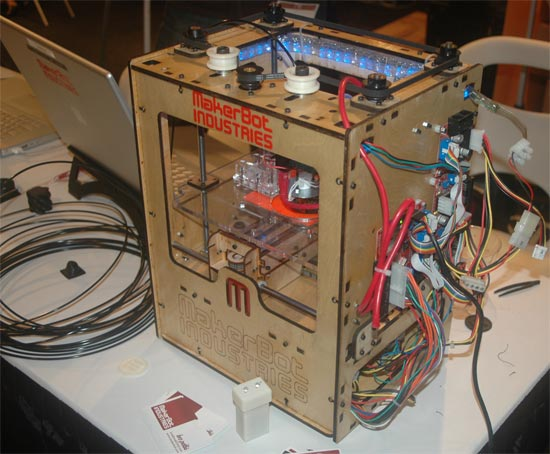
\includegraphics[width=.4\linewidth]{images/makerbot}&
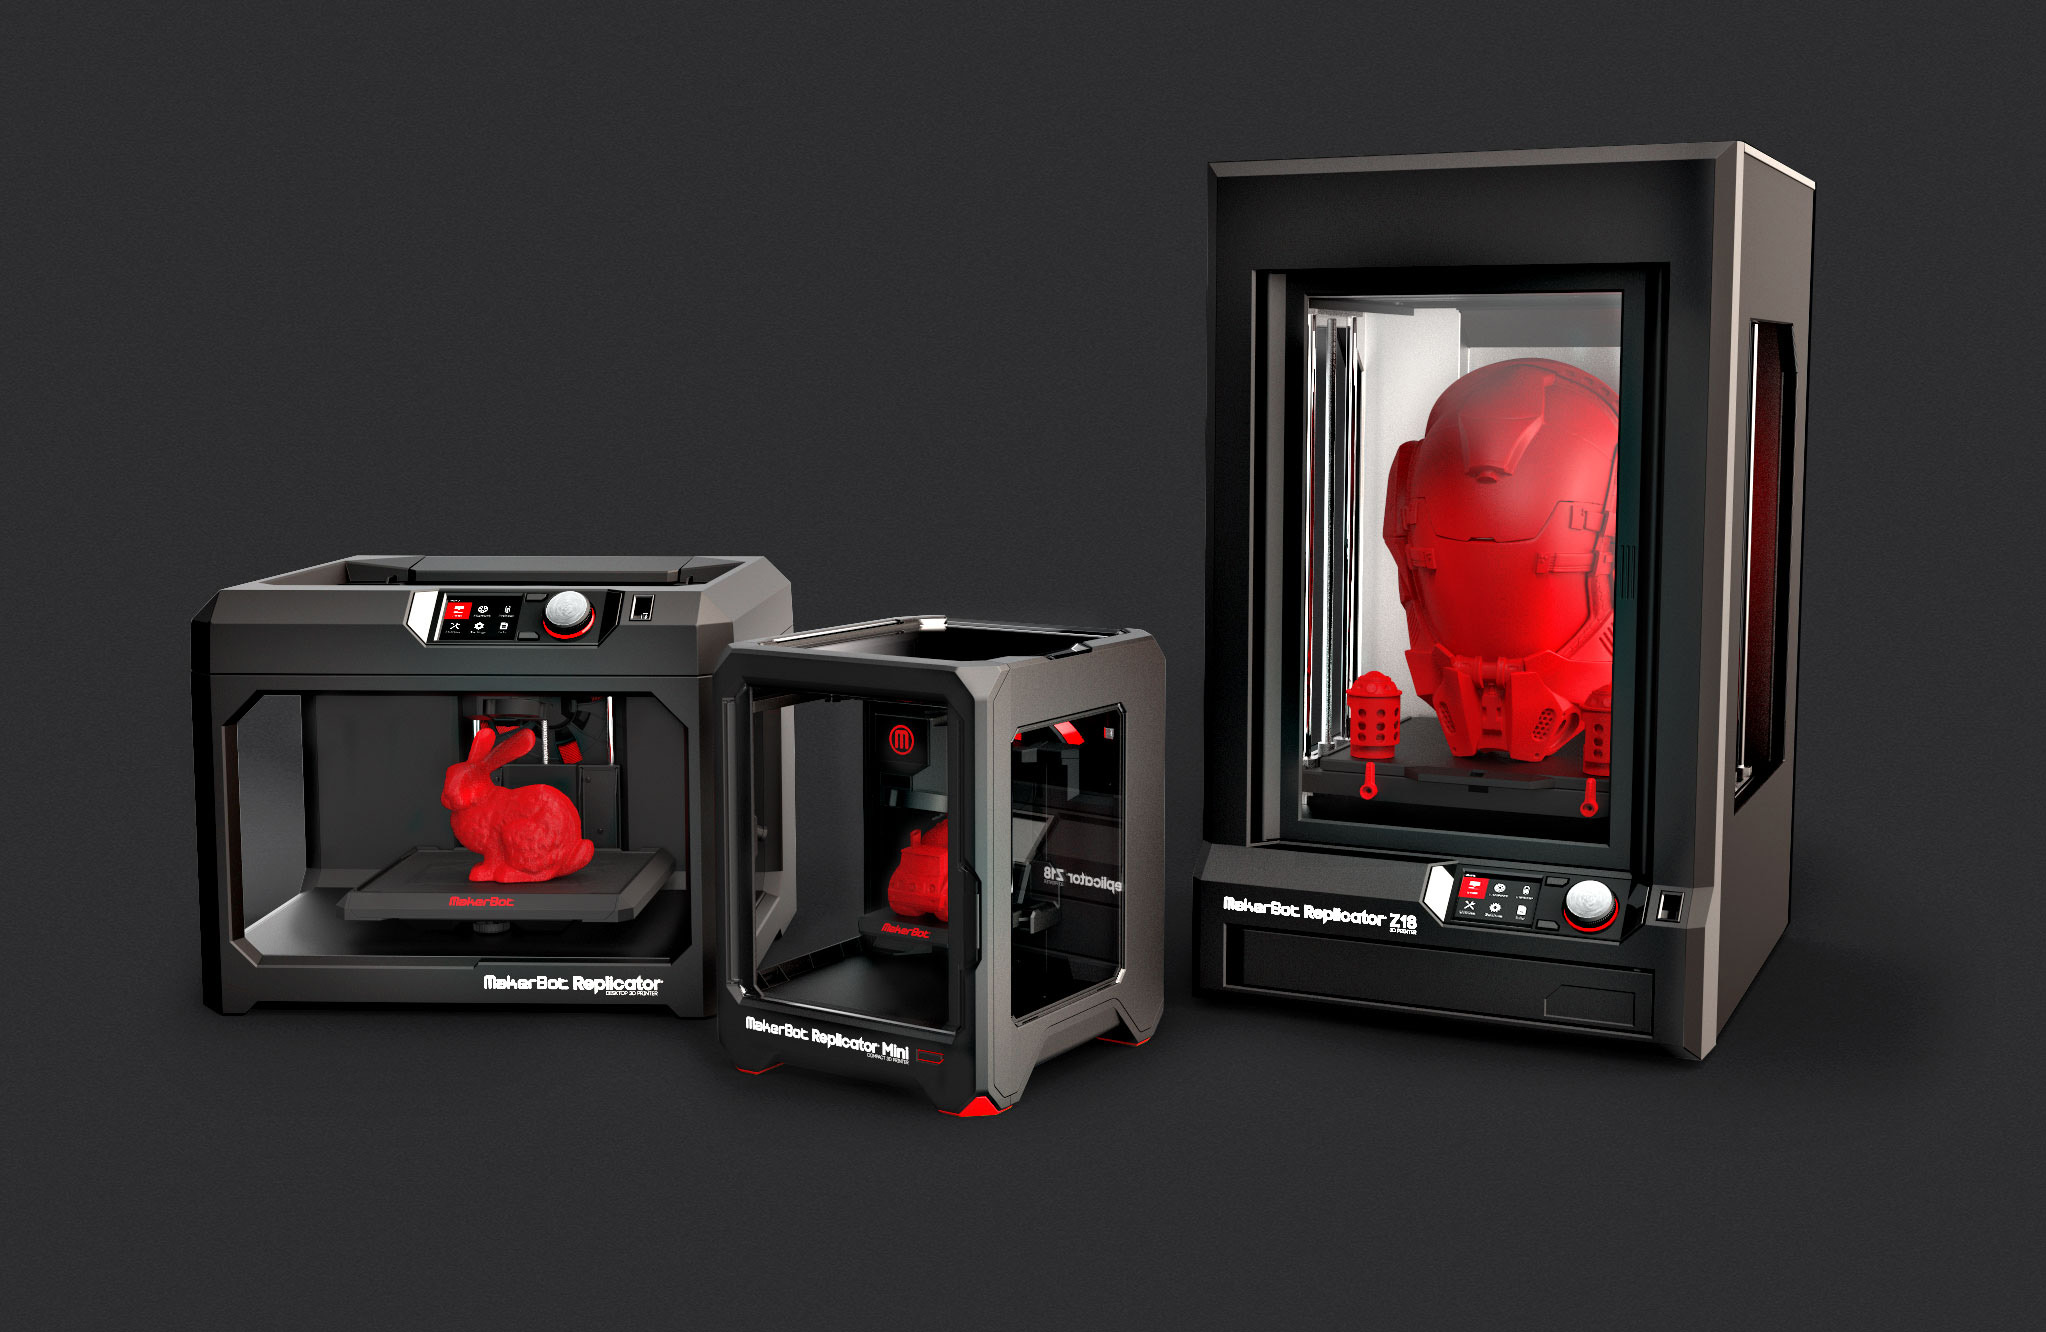
\includegraphics[width=.5\linewidth]{images/MB05_REP_Group}
\end{array}$
\end{center}
\caption{Left: One of the first popular desktop 3D printers, the MakerBot
``Cupcake CNC'', released in 2009. Right: The latest group of MakerBot models,
released at the Consumer Electronics Showcase in January 2014.}
\label{makerbot}
\end{figure}

Although printing out dozens of army men or barnyard animal figurines may be
satisfying for a time, and indeed speaks to the compelling nature of 3D
printing, it seems fair to say that children do not learn much about 3D modeling
from a ``download and print'' paradigm. Herein lies the crux of the problem - 3D
printing offers a wonderfully rich new platform for design, creativity, and
exploration, but neither the 3D printer manufacturers nor the companies who
produce the software necessary to author files suitable for 3D printing have
made accessibility for novices a priority. This is where our journey begins:
the desire to democratize 3D printing in a way that empowers newcomers,
particularly youngsters, in designing their own objects for 3D printing;
engaging them in such a way that intuitively introduces many of the core
concepts of 3D modeling, while helping to solidify cognitive processes around
spatial reasoning and 2D/3D translations, by building a set of devices that act
as a new genus amongst an ecosystem of next-generation digital fabrication
interfaces.

How, then, did we arrive at the term ``embodied fabrication'' to describe this
new genus? The simple answer, at the risk of over-extending the genealogical
metaphor, is that we selected what we deemed to be the best, most relevant
traits from a number of related areas (computer science, cognitive science,
developmental psychology, pedagogical theory, and digital fabrication
technology, amongst others) and attempted to splice them together in such a way
as to meaningfully address the issues with 3D printing outlined above. 

We derive the term ``embodied'' from cognitive science, and the fairly recent
advances in an area known as ``embodied cognition''. Embodied cognition posits
that our physical bodies and their interactions with the world are more closely
bound to our cognitive processes than previously thought. Evidence from research
in this area (discussed more thoroughly in Chapter 3 on related work) points to
cognitive benefits in basic arithmetic, ratios, proportions, and spatial
reasoning - all of which are useful (if not essential) tools in 3D modeling,
simply by involving the body more closely in the learning process.
This evidence, combined with the simple intuition that learning the skill of
3-dimensional modeling ought to be done in 3-dimensions as much as possible and
not solely on a 2-dimensional screen, provided the impetus for us to look toward
a physical solution that involves the body more than a typical piece
of software.

Physical, or ``tangible'' user interfaces are nothing new; wooden blocks have
been a part of children's education in a pedagogical sense since the beginning
of kindergarten over 150 years ago\cite{froebel}. Montessori ``manipulatives''
developed in the early part of last century inspired some of the first attempts
at creating physical, computationally-enhanced construction kits for children in
the 1980's\cite{Resnick:1998:DMN:274644.274684}. Tangible user interfaces, or
TUIs have been a growing part of human-computer interaction in a formal way
since Hiroshi Ishii's work on ``tangible
bits''\cite{Ishii:1997:TBT:258549.258715} in the mid 1990's, and of course the
influence of icons such as Doug Engelbart\cite{engelbart1968research} - one
might argue the mouse was the first ``embodied'' peripheral for a computer, in
the 1960's - and Mark Weiser\cite{weiser1991computer} (who presaged many of the
devices we take for granted today) as well as many others, should not be
overlooked - we give a more detailed account of this lineage when discussing
related work. For us, the longevity, breadth of applications, and numerous
achievements of mediating human-computer interaction though different physical
interfaces further suggests that a tangible user interface, coupled with the
proper software is more than capable of providing an accessible and embodied
foundation for our work.

Taking design principles from the lexicon of tangible user interfaces, adapting
them to better fit an embodied cognition world-view, and focusing on enabling 3D
modeling specifically for 3D printers, we designed and built a suite of
functional prototype devices for an embodied mode of digital fabrication; hence
the title of our work. To this end, we present a class of tangible user
interfaces designed to scaffold a child's ability to design, explore, and play
in three dimensions, with a particular focus on enabling original output for 3D
printing. We present three prototype devices (called UCube, SnapCAD,
and PopCAD) as well as piece of companion software that translates the physical
actions performed on the devices into screen-based content in real-time.

To give a brief preview of our creations; with their hands, users manipulate a
device to specify points (as coordinates in 3-space) that simultaneously display
as active dots against a ghosted 3D grid in real-time on a computer. The
software on the computer allows for certain modeling operations on this set of
input points (e.g., taking the convex hull, making a path through space),
exporting shapes to stereolithography (.STL) format with the click of a button,
the preferred format for 3D printers, as well as other functionality that we
explore more thoroughly in the next chapter.

We propose that these designs form a novel class of embodied input devices aimed
at enabling novice output for digital fabrication machines. Over three separate
user studies with 11 to 18 year olds, we investigate the ability for children to use
our devices to model a given shape (with and without the companion software) and
to match configurations on our device to a printed 3-dimensional object (without
the aid of the software). In our last study we compare two of our devices over a
multi-session study, while also administering a set of spatial reasoning tasks
as a pre and post test. We video record the subjects (with parental consent)
and analyze the gesture and speech expressions the participants make when
explaining a modeling strategy to reproduce a given object.

Through our studies, we show evidence that our suite of devices can be used
effectively by young adolescents with very minimal instruction, that a wide
variety of shapes can be recreated by the majority of subjects who used our
devices, that spatial test scores and modeling performance tends to improve over
multiple sessions with our devices, and that the kinds of gestures produced
while explaining modeling strategy correlates to modeling success on our
devices, a finding which supports prior research on gesture analysis by other
authors.

By providing a feedback loop between the bodily interaction with
tangible interfaces and the observed changes in real-time on a computer screen,
this body of work presents strong new motives for the inclusion of embodied
cognition in tangible interface design, while tackling the lack of appropriate
tools for novices to create for 3D printers, and evaluating the efficacy of our
devices as modeling tools and as devices for strengthening spatial reasoning and
cognition. We continue in Chapter 2 to present our prototype devices and the
software they operate with, explaining the evolution of our design choices as
well as the technical details behind their operation. Chapter 3 details the lineage
of related work, hinted at somewhat in this introduction, drawing connections
between the childhood developmental theories and conceptions of space developed
by Piaget and refined by Papert, the notions of cognitive development and
embodied mathematics discussed by Lakoff and Nu\~nez, the democratization of
digital fabrication technologies discussed by Gershenfeld and Lipson, and the
previous adaptation of these achievements into computer science. Chapter 4 is
devoted to the evaluation of our work, presenting three user studies, their
procedures and results. Chapter 5 delves deeper into the discussions which
surround the observations from our studies, comparing them with prior research,
and against each other. Finally, Chapter 6 provides a vision for immediate
future work on our devices, a more expansive vision of the possibilities
inherent in embodied fabrication, and ends with our concluding thoughts.



% The work presented here draws on the stages of childhood developmental theories
% and conception of space developed by Piaget and refined by Papert, notions of
% cognitive development and embodied mathematics discussed by Lakoff and Nu\~nez,
% the democratization of digital fabrication technologies discussed by Gershenfeld
% and Lipson, and the previous adaptation of these achievements into computer
% science.
























%old intro
% Digital fabrication technologies are increasingly finding their way into
% educational spaces of all shapes and sizes. These new technologies 
% (3D printers, laser cutters, etc.) afford opportunities for exploring these new
% ways of `making' and how they may change the way we learn, explore, and play.
% Although there is much excitement surrounding the `maker movement' - and 3D
% printing in particular - there has been little examination of how to introduce
% a younger audience to 3D printing in an empowering way.
% This proposal argues that tangible interfaces - as opposed to 2D screen-based
% media - can be designed not only to support spatial reasoning and mathematical
% intuitions in children by engaging them in exploratory modeling and play, but
% that these interfaces can act as a democratizing force by enabling children to
% create physical objects with digital fabrication devices.
% The proposed work presents a series of novel tangible input devices for
% enhancing mathematical and spatial reasoning in kids with a focus on generating
% output for 3D printing. We discuss related work, the status of the proposed
% work, additional improvements to be made, a timeline for completion,
% and a discussion of risks, limitations, and outcomes inherent in the proposal.
% 
% 
% %from proposal
% A number of computer scientists, technologists, and educators have declared that
% the era of personal fabrication is upon
% us\cite{anderson2012makers}\cite{Gershenfeld:2007:FCR:1211574}. New devices
% aimed at increasing the ability of the individual to physically manufacture
% their own ideas are being released at breakneck speed. The cultural and
% technological shifts caused by this change are taking many forms, yet few
% technologies associated with the `maker' movement have received as much
% attention as 3D printing - the ability (by various means) to digitally design
% and then print out physical 3-dimensional objects. Media outlets from
% Forbes\cite{forbes} to The Economist\cite{economist} have extolled the
% disruptive and democratizing possibilities that 3D printing offers - at least as
% it affects the traditional manufacturing supply chain. Less examined has been
% how to introduce novices, specifically pre-teens and early adolescents, to 3D
% printing - and perhaps more importantly - discussing what (and how) they might
% learn by being exposed to it.
% While the variety of desktop 3D printers continues to increase and the cost of
% adding a `fab lab' of digitally-based manufacturing tools in the home or
% classroom steadily declines, the types of interfaces by which children can
% easily and intuitively design and explore the capabilities of 3D printers still
% remains a barren landscape consisting primarily of software-only solutions. It
% is this landscape that we are interested in seeding, following the best
% practices in computational and cognitive science with particular attention to
% children-centered design.




% \section{A Brief Overview of this Thesis}
% 
% \section{Motivations}
